% Two independently chosen child types: seven boy-days then seven girl-days.
% Columns = older child, rows = younger child. Index 1 = boy born on Tuesday.
% Highlighted cross: 14 + 14 - 1 = 27 cases, of which 7 + 7 - 1 = 13 have two boys.
% Exact finite sample space, not a simulation. 14 x 14 equally likely cells.
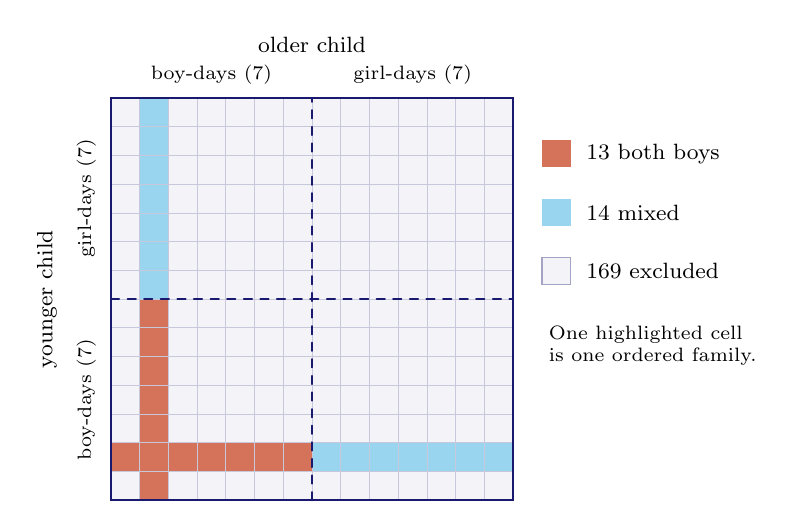
\begin{tikzpicture}[x=0.365cm,y=0.365cm,line cap=round]
  \fill[MidnightBlue!5] (0,0) rectangle (14,14);
  % One Tuesday boy in the older-child or younger-child coordinate.
  \fill[SkyBlue!85] (1,0) rectangle (2,14);
  \fill[SkyBlue!85] (0,1) rectangle (14,2);
  % Cases with two boys, among the highlighted Tuesday-boy cases.
  \fill[BrickRed!55] (1,0) rectangle (2,7);
  \fill[BrickRed!55] (0,1) rectangle (7,2);
  \draw[step=1,MidnightBlue!24,line width=0.3pt] (0,0) grid (14,14);
  \draw[MidnightBlue,thick] (0,0) rectangle (14,14);
  \draw[MidnightBlue,dashed,line width=0.7pt] (7,0)--(7,14) (0,7)--(14,7);
  \node[font=\scriptsize,anchor=south] at (3.5,14.15) {boy-days (7)};
  \node[font=\scriptsize,anchor=south] at (10.5,14.15) {girl-days (7)};
  \node[font=\scriptsize,rotate=90,anchor=south] at (-0.18,3.5) {boy-days (7)};
  \node[font=\scriptsize,rotate=90,anchor=south] at (-0.18,10.5) {girl-days (7)};
  \node[font=\footnotesize,anchor=south] at (7,15.25) {older child};
  \node[font=\footnotesize,rotate=90,anchor=south] at (-1.55,7) {younger child};
  \fill[BrickRed!55] (15,11.6) rectangle (16,12.55);
  \node[font=\footnotesize,anchor=west] at (16.2,12.05) {$13$ both boys};
  \fill[SkyBlue!85] (15,9.55) rectangle (16,10.5);
  \node[font=\footnotesize,anchor=west] at (16.2,10.02) {$14$ mixed};
  \fill[MidnightBlue!5] (15,7.5) rectangle (16,8.45);
  \draw[MidnightBlue!40] (15,7.5) rectangle (16,8.45);
  \node[font=\footnotesize,anchor=west] at (16.2,7.97) {$169$ excluded};
  \node[font=\scriptsize,align=left,anchor=north west] at (14.9,6.4) {One highlighted cell\\is one ordered family.};
\end{tikzpicture}
